\documentclass[a4paper,14pt]{extarticle}
\usepackage{cmap}				% To be able to copy-paste russian text from pdf			
\usepackage[utf8]{inputenc}
\usepackage[T1]{fontenc}
\usepackage[margin=1in]{geometry}
\usepackage[english, russian]{babel}

\usepackage[hyphens]{url}
\urlstyle{same}
\usepackage{hyperref}

\usepackage{multirow}
\usepackage{graphicx}
\usepackage{caption}
\usepackage{amsmath}
\usepackage{mathtools}

\usepackage{tikz}
\usepackage{pgfplots}
\usepgfplotslibrary{groupplots,colorbrewer,dateplot,statistics}

%\def\ishtml{1}
\ifdefined\ishtml
  % HTML mode
  \newcommand{\urlnote}[2]{\href{#2}{#1}} % Make cool link 
  \newcommand{\smallsep}{thinspace} % to be replaced with unicode 8239 later
\else
  % PDF mode
   \usepackage{libertine}
   \usepackage{libertinust1math}
   \newcommand{\urlnote}[2]{#1\endnote{\url{#2}}}  % Put URLs to endnotes
   \newcommand{\smallsep}{\kern 0.1em}
\fi

% Move footnotes to end of document
\usepackage[backref=true]{enotez}
\DeclareTranslation{russian}{enotez-title}{Примечания}

\usepackage[
	output-decimal-marker={,},
	group-separator={\smallsep},
	group-minimum-digits=3
]{siunitx}

% Shoot me if I know a better way to make decimal groups of two
\newcommand{\rateone}[1]{\num{#1}}
\newcommand{\ratetwo}[2]{\num{#1}\smallsep#2}
\newcommand{\ratethree}[3]{\num{#1}\smallsep#2\smallsep#3}

\newcommand{\ru}[1]{\begin{otherlanguage}{russian}#1\end{otherlanguage}}
\newcommand{\en}[1]{\begin{otherlanguage}{english}#1\end{otherlanguage}}
\newcommand{\ruen}[2]{#1 (\en{#2})}

\usepackage[style=alphabetic, backend=biber]{biblatex}
\addbibresource{index.bib}
\renewcommand*{\bibfont}{\small}
\setcounter{biburllcpenalty}{9000}
\setcounter{biburlucpenalty}{9500}

\author{Артём Бакулин}
\date{\today}
\title{Снегоходы, пиво и деривативы на погоду}

\begin{document}

\maketitle
\thispagestyle{empty}

\begin{figure}[h]
\centering
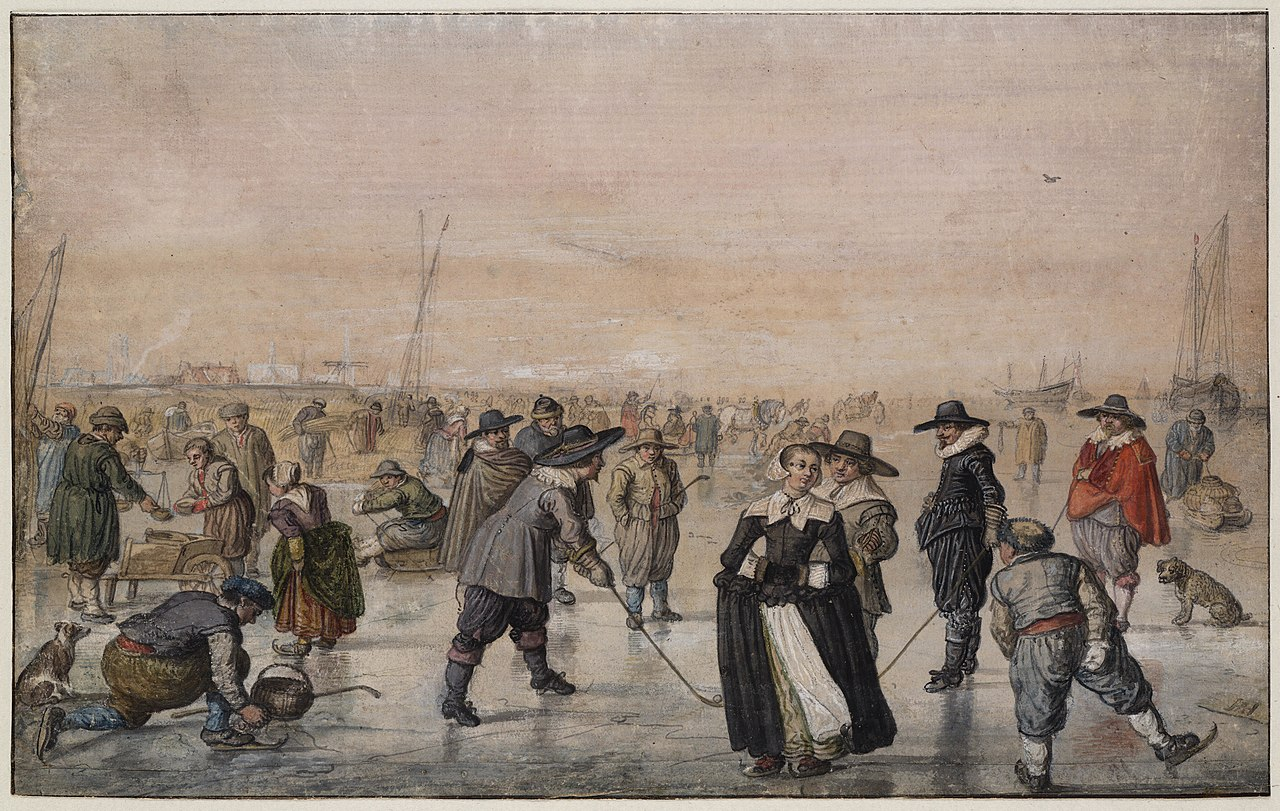
\includegraphics[width=\textwidth]{a_scene_on_the_ice.jpg}
\captionsetup{labelformat=empty}
\caption{\small{
Хендрик Аверкамп. \urlnote{Сцена на льду}
{https://commons.wikimedia.org/wiki/File:Hendrick_Avercamp_-_A_Scene_on_the_Ice_-_WGA01076.jpg}.
ок. 1615--1630 г. Музей Тейлора, Харлем.
}}
\end{figure}
\newpage

\section*{Введение}

Канадская компания Bombardier, известная нам своими самолётами, помимо всего
прочего производит и снегоходы. Собственно, со снегоходов всё и началось, когда
в 30-е годы прошлого века Жозеф-Арман Бомбардье разработал первые серийные
образцы.

В конце 90-х годов продажи снегоходов в Северной
Америке застопорились и упорно отказывались расти. Маркетологи выяснили
очевидную, в принципе, вещь. Потенциальные клиенты отказывались от покупки,
потому что опасались тёплой зимы без снега. Мало кому понравится выложить
кругленькую сумму за игрушку, которая потом простоит в гараже весь первый сезон по
милости матушки-природы.

Казалось бы, ничего не поделаешь. Погода --- совершенно непредсказуемая штука,
повлиять на которую не под силу ни самой Bombardier, ни тем более розничным
покупателям. Остаётся только читать пугающие новости о глобальном потеплении и
готовиться к тому, что дальше будет только хуже. На помощь пришла финансовая
инновация, последний писк моды --- деривативы на погоду, то есть контракты, платежи
по которым зависят от метеоусловий.

\section*{Деривативы на снегопад}

Bombardier предложила клиентам страховку. Если в год покупки снегохода зима выдастся
малоснежной (снега выпадет меньше, чем половина среднего за три последних года в
данной местности), то весной обескураженный покупатель автоматически получит от компании чек
на \$\num{1000}, чтобы деньги скрасили ожидание следующей зимы. Сумма
достаточно солидная, учитывая, что топовая модель снегохода стоила примерно
\$\num{10000}, а бюджетные продавались по \$\num{3000}. Это была бомба: в
первый год продажи выросли на 38\%!

Разумеется, никто, включая Bombardier, не умеет предсказывать погоду на месяцы
вперёд. Было бы слишком опрометчиво сидеть сложа руки и гадать, придётся ли
выплачивать компенсации покупателям.

Bombardier заключила сделку с энергетической компанией Enron, одним из пионеров рынка погодных деривативов. На каждый проданный
снегоход Bombardier платила Enron от \$40 до \$450 в зависимости от города, в котором
жил покупатель снегохода. Взамен Enron брала на себя обязательство выплатить Bombardier те
самые \$\num{1000}, если зима окажется малоснежной \cite{wsj1999}. Благодаря этой сделке
Bombardier не рисковала неожиданно разориться из-за тёплой зимы. 

Сделка между Bombardier и Enron --- классический пример дериватива на погоду. В общем случае,
чтобы договориться о погодном деривативе, две стороны сделки должны выбрать
базовый показатель (например, количество снега, выпавшего на
конкретной метеостанции), период наблюдения (например, три зимних месяца) и
формулу, по которой можно вычислить итоговую выплату из базового
показателя (например, \$\num{1000}, если снега меньше, чем половина среднего за три последних года, либо \$0 в противном случае).

\section*{Перераспределение риска}

На первый взгляд, в результате сделки ничего не изменилось, потому что
неопределённость, связанная с будущей погодой, не исчезла. По-прежнему никто из
смертных не знал, сколько снега выпадет предстоящей зимой. Кроме того, если вы
привыкли смотреть на финансовый рынок как на игру с нулевой суммой, то вы могли
увидеть знакомые черты и в этой ситуации, потому что потенциальная прибыль
покупателя снегохода равна убытку Bombardier, а прибыль Bombardier равна убытку
Enron.

Тем не менее, произошла незаметная, но важная вещь. Деривативы позволили перераспределить
риск между участниками схемы. Если раньше от малоснежной зимы страдал только невезучий
покупатель снегохода, то теперь он мог рассчитывать на компенсацию от Bombardier, которая, в
свою очередь, переложила риск на Enron.

Одно лишь перераспределение риска изменило поведение людей, которые всё-таки
решились осуществить мечту и купить снегоход. \en{Bombardier}\ значительно нарастила продажи, и рост
выручки с лихвой окупил расходы на сделку с Enron. Наконец, поскольку зимой 98/99 выпало
достаточно снега, Enron не пришлось выплачивать компенсации, и она смогла
неплохо заработать. Все счастливы. Настоящее волшебство, не правда ли?

<<Постойте! --- воскликнет читатель, --- а что если бы зима оказалась малоснежной? Ведь Enron
понесла бы убытки!>> В самом деле, Enron заработала, потому что продала страховку от
события, которое так и не случилось. Ну так это же и есть бизнес-модель страховых компаний со
времён Вавилона. Надо полагать, аналитики Enron рассчитали вероятность малоснежной зимы
и выставили такую цену страховки, чтобы в среднем не остаться в убытке.

Впрочем, Enron могла бы не оставлять риск у себя, а переложить его на кого-то
ещё. Для этого нужно было бы найти кого-то, кто имеет противоположную
чувствительность к погодному риску --- того, чьи дела идут лучше, когда снега мало,
и хуже, когда снега много. Кто бы это мог быть? Фермер, у которого в случае тёплой
зимы лучше урожай озимых. Муниципалитет, который не тратит деньги на расчистку
улиц. Сами жители, которым не приходят гигантские счета за отопление. Можете
продолжить список сами.

Предположим, что некий фермер купил у Enron страховку от морозной (а не от тёплой!)
зимы. Тогда Enron получит страховую премию и от Bombardier, и от фермера. Если зима
окажется тёплой, то деньги фермера пойдут на выплаты Bombardier, которая передаст их
покупателям снегоходов. Если зима будет холодной, то Enron компенсирует убытки фермера
за счёт денег, полученных от Bombardier.

\section*{Неприятие риска и потерь}

Если убрать из цепочки перераспределения риска
посредников, \en{Bombardier}\ 
и \en{Enron}, то выходит, что покупатель снегохода застраховал фермера
от холодной зимы, а фермер в ответ застраховал покупателя снегохода от тёплой зимы. Интересно, что эта сделка может быть выгодна обоим! Дело в том, что люди не любят неопределённость и ещё больше не любят убытки.

Чтобы проверить, насколько вы не любите неопределённость, поставьте мысленный эксперимент. Представьте, что вас заперли в подвале и предлагают выбрать из двух вариантов. Во-первых, можно просто заплатить \$10 и выйти из подвала. Во-вторых, можно сыграть в орла и решку на \$\num{10000} с шансами 50/50. Независимо от того, выиграете вы или проиграете, после игры вас тоже отпустят. 

Чисто математически, средний выигрыш в орлянке равен \$0, и это может показаться выгоднее, чем верная потеря \$10. Однако, скорее всего вы предпочтёте наверняка потерять \$10, а не подбрасывать монетку, поскольку возможная радость от выигрыша \$\num{10 000} не перевешивает возможную тоску от потери \${10 000}.

Не исключено, что вы согласитесь гарантированно потерять даже не \$10, а все \$100 или \$500, лишь бы не играть в орлянку. Конкретная сумма, которую вы будете готовы заплатить, зависит от вашей личной чувствительности к риску и потерям. Экономисты называют этот эффект \ruen{неприятием риска}{risk aversion} и \ruen{неприятием потерь}{loss aversion}.

Если вы уже отошли от жестокого мысленного эксперимента, то применим полученное знание к гипотетической сделке покупателя снегохода и фермера.

Покупатель снегохода не так радуется выпавшему снегу, как расстраивается от бесснежной зимы. Фермер не так радуется дополнительному урожаю в тёплую зиму, как расстраивается из-за неурожая, вызванного неожиданными морозами. Они оба заинтересованы в том, чтобы ограничить свои убытки в случае неблагоприятного стечения обстоятельств, поэтому вполне могли бы договориться застраховать друг друга. Это возможно, потому что плохой сценарий для одного одновременно является хорошим сценарием для другого, и наоборот.

\section*{Деривативы и страховые полисы}

Возможность заключить сделку с кем-то, имеющим противоположную чувствительность к риску --- главное отличие финансовых деривативов (не только погодных) от страховок,
хотя между ними, действительно, много общего.

Когда страховая компания продаёт вам
полис, скажем, от пожара, вряд ли она рассчитывает после этого продать кому-то полис от
\emph{отсутствия} пожара. Риск остаётся у страховой компании, и если пожаров будет
слишком много, то она разорится. Например, один из переломных моментов сюжета <<Финансиста>>
Теодора Драйзера --- великий пожар в Чикаго, который привёл к банкротству страховых
компаний и обвалу фондового рынка.

Деривативы, по крайней мере отчасти, избавлены от этого недостатка. Если фермеру
пришлось выплачивать страховку покупателю снегохода, то это означает, что зима
была тёплой, фермер собрал хороший урожай и скорее всего не испытывает финансовых
проблем. Конечно, фермер может разориться и по причинам, не имеющим отношения к
погоде. Поэтому для большей надёжности многие деривативные сделки проходят с
участием центральных контрагентов (о которых вы можете прочитать в \urlnote{предыдущей статье}{https://habr.com/ru/company/dbtc/blog/467415/})
или требуют внесения залога.

Впрочем, если на рынке деривативов на валюту или нефть почти всегда есть участники с
противоположными интересами, то на рынке деривативов на погоду всё не так просто.
Часто у продавца страховки нет возможности заключить противоположную сделку с кем-то другим,
и ему остаётся только гадать, не преподнесёт ли погода неприятный сюрприз. Enron
в своё время повезло со снежной зимой, но история знает и примеры невезения.

\section*{Деривативы для любителей пива}

В начале 2000-х годов организаторы фестиваля пива Октоберфест в Мюнхене справедливо
рассудили, что в дождливую погоду люди более склонны остаться дома, и посещаемость
фестиваля снижается. Организаторы обратились за страховкой в один крупный немецкий банк из Франкфурта. Договорились, что если в течение двух недель
фестиваля дождь будет идти более четырёх дней, то банк выплатит компенсацию за пятый
и каждый последующий дождливый день.
 
У банка не было никаких шансов заключить обратную сделку с кем-то ещё.
Действительно, кто в здравом уме будет страховаться от сухой погоды в начале
осени? Фермер, который внезапно испугается сорокоградусной засухи в октябре?
Организаторы фестиваля любителей проливных дождей? В общем, банку пришлось
выступить в роли страховой компании и оставить риск у себя.

Команда аналитиков раздобыла метеосводки Мюнхена за сотню с лишним лет и
вычислила стоимость страховки, которая позволила бы банку не остаться в минусе.
Как вы можете догадаться, что-то пошло не так. Разверзлись хляби, и потоп смыл
Октоберфест 2002-го года. Количество дождливых дней превысило исторический рекорд,
и банк заплатил любителям пива существенно больше, чем рассчитывал \cite[p.~160]{rodgers2016why}.

\section*{Заключение}

Если в экономике есть два субъекта с противоположной чувствительностью
к какому-то риску, будь то будущий курс валюты или толщина снежного покрова, то они
могут договориться о деривативе, то есть согласиться поделиться частью прибыли
в хорошем сценарии в обмен на компенсацию убытков в плохом сценарии.

Неприятие потерь и желание избежать риска глубоко вшито в человеческую
психику, поэтому одно лишь перераспределение риска может сделать участников сделки
счастливее. Как минимум, они будут крепче спать. Как максимум, новое распределение
риска изменит их потребительские и инвестиционные решения и будет способствовать
экономическому росту. Вспоминайте об этом каждый раз, когда вас будут убеждать, что
деривативы --- это всего-навсего игра с нулевой суммой для спекулянтов.

К сожалению, не обойтись без ложки дёгтя. Как вы, возможно, слышали, в 2001-м году
Enron с треском разорилась и попутно утянула за собой аудиторскую фирму Arthur
Andersen. Выяснилось, что руководство Enron весьма творчески подходило к
финансовому учёту, за что получило длительные тюремные сроки. Кто знает, если бы
зима 98/99 оказалась тёплой, то с Enron сталось бы спрятать убытки, и вдохновляющая
история со снегоходами оказалась бы всего лишь очередным эпизодом громкого уголовного дела.

\section*{Дальнейшее чтение}

Если вам интересно, как мы мыслим и принимаем решения, то обязательно прочитайте
книгу одного из основоположников поведенческой экономики Даниела Канемана 
<<Думай медленно... Решай быстро>> \cite{kanheman2013think}. Неприятие риска и
потерь --- лишь одна из многих особенностей нашего мозга, выработанных эволюцией.

\section*{Отказ от ответственности}

Мнение автора статьи может не совпадать с официальной позицией Deutsche Bank AG.
Статья не является предложением или рекламой какой-либо услуги. Упоминание
третьих сторон не предполагает одобрения или неодобрения. Автор и Deutsche Bank
напоминают, что торговля на финансовых рынках сопряжена с риском, и не несут
ответственности за возможные негативные последствия ваших личных инвестиционных
решений.

\begin{otherlanguage}{english}
\printbibliography[title = \begin{otherlanguage}{russian}Список
литературы\end{otherlanguage}]
\end{otherlanguage}

\printendnotes

\end{document}
